\section[Closing]{Closing thoughts}
\label{sec:closing}

%---------------------------------------------------------------
% 1. Summary
%---------------------------------------------------------------
\begin{frame}{Seminar summary}

	\begin{columns}[c]
		% lessons
		\begin{column}{.45\textwidth}
		    You've learned:
		    \begin{itemize}
			    \item What intellectual property is
			    \item How licenses can help you 
			    \item How openness doesn't stop you making money
			    \item That you need to get a lawyer involved.
		    \end{itemize}
		\end{column}

		\begin{column}{.45\textwidth}
		
		    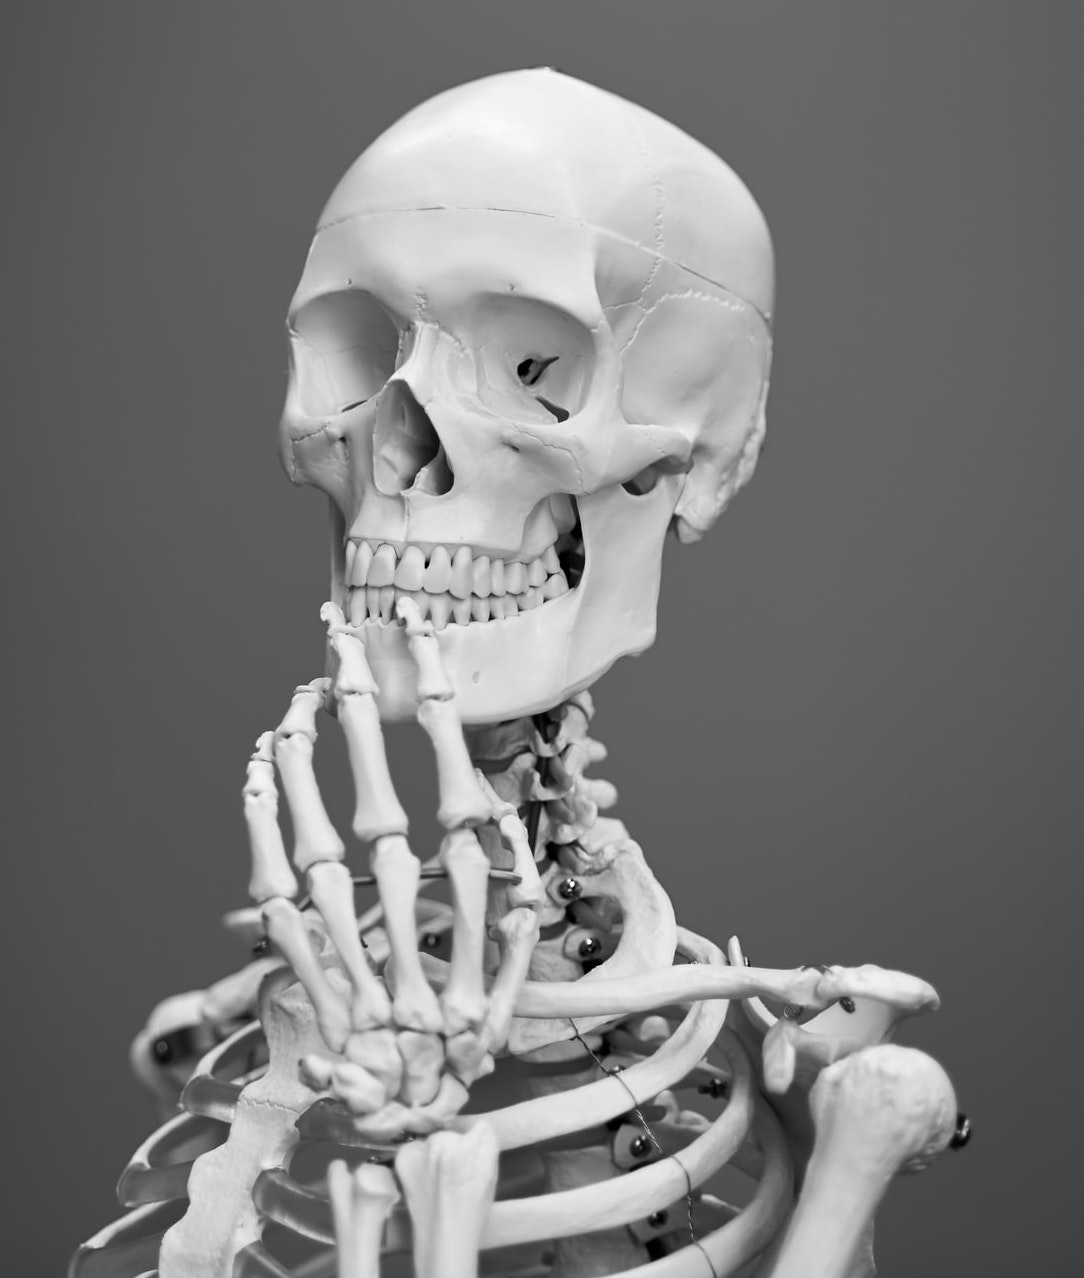
\includegraphics[width=0.85\textwidth]{images/mathew-schwartz-8rj4sz9YLCI-unsplash-crop.jpg}
		    
		    \givecredit{%
		        \centering
		        Photo by \textlink{https://unsplash.com/@cadop}{Mathew Schwartz} on \textlink{https://unsplash.com/s/photos/thinking}{Unsplash}}
		\end{column}
		
	\end{columns}

\end{frame}

%---------------------------------------------------------------
% 2. Next steps
%---------------------------------------------------------------

\begin{frame}{What to do now}

	\begin{columns}[t]
		\column{.45\textwidth}
		
		\begin{block}{Further reading}
		\begin{itemize}
		    \item \textlink{https://www.linux.com/news/birth-linux-how-linux-got-started/}{The Birth of Linux: How Linux Got Started.} (Linux.com, 2020)
		    \item \textlink{http://openbikeinitiative.org/}{The open Bike Initiative}
		\end{itemize}
		\end{block}
		
		\begin{block}{Self-study 3: Implementing Open Science}
			Working with your group, implement at least two of the ideas you identified in self-study 2.
			\begin{itemize}
			    \item See the \textlink{https://github.com/LIKE-ITN/OpenScienceTrainingCourse/tree/master/06_selfstudy3}{guidance on GitHub}.
			\end{itemize}
		\end{block}

		\column{.45\textwidth}
		\begin{block}{Seminar 4: communicating your science}
			Selling your brand and research through social media, professional networks, etc., and other strategies to make people aware of your work.
			\begin{itemize}
				\item See the \textlink{https://github.com/LIKE-ITN/OpenScienceTrainingCourse/blob/master/07_seminar4/readme.md}{Seminar materials on GitHub}
			\end{itemize}
		\end{block}

	\end{columns}

\end{frame}

%---------------------------------------------------------------
% 3. Let's make this open
%---------------------------------------------------------------
\begin{frame}{Let's make this presentation open}

	\begin{columns}[t]
		\begin{column}{.45\textwidth}
		    \centering
		    
\includegraphics[height=1.5cm]{images/1280px-FAIR_data_principles.jpg}

		    \givecredit{\centering Image source: \textlink{https://en.wikipedia.org/wiki/FAIR_data#/media/File:FAIR_data_principles.jpg}{Wikimedia}. Credit: \textlink{https://commons.wikimedia.org/w/index.php?title=User:SangyaPundi}{SangyaPundir}. \\
		    Reused under the \textlink{https://creativecommons.org/licenses/by-sa/4.0}{CC BY-SA 4.0 license}}
		\end{column}

		\begin{column}{.45\textwidth}
		    \centering
		    
\includegraphics[height=1.5cm]{images/cc-by-sa.png}
        \end{column}
	\end{columns}

	\begin{columns}[t]
		\begin{column}{.45\textwidth}
		    \centering
		% Findable
		    \begin{block}{Findable}
			    This presentation has a DOI:
		    \end{block}

		    % accessible
		    \begin{block}{Accessible}
			    This presentation is archived at Zenodo.org. \\
			    The source code is available through GitHub.
		    \end{block}
        \end{column}

		\begin{column}{.45\textwidth}
		    \centering
		    \begin{block}{Interoperable}
			    This material is produced using the \LaTeX\space `Beamer' package.
		    \end{block}

		    \begin{block}{Reusable}
			    This material is reusable under the \textlink{https://creativecommons.org/licenses/by/4.0/}{CC-BY-4.0 license}.
		    \end{block}
        \end{column}
	\end{columns}
\end{frame}